%=========================================================================
%  Paste this whole file into a new Overleaf project (main.tex) and add the
%  refs.bib file from this folder. Compiler: pdfLaTeX. IEEEtran is built into
%  Overleaf.
%
%  Target: Journal of Autonomous Agents and Multi-Agent Systems (JAAMAS), 2027.
%  JAAMAS uses the Springer format for the camera-ready; this IEEE draft is for
%  circulation and the capstone panel.
%
%  Results are 3 training seeds x 10 held-out eval seeds (scripts/run_all.py).
%  The E5 robustness table is filled from scripts/run_ablations.py.
%=========================================================================
\documentclass[conference]{IEEEtran}
\IEEEoverridecommandlockouts
\usepackage{cite}
\usepackage{amsmath,amssymb,amsfonts}
\usepackage{graphicx}
\usepackage{booktabs}
\usepackage{siunitx}
\usepackage{xcolor}
\usepackage[hidelinks]{hyperref}

\begin{document}

\title{Policing the Data It Creates: Feedback and Fairness in a\\
Reinforcement-Learned Patrol-Allocation Rule over an\\
Unseeded Crime Simulator}

\author{
\IEEEauthorblockN{Ashmith Reddy Sama, Dennis Philip, Dhrithi Kiran, Diya Saigal}
\IEEEauthorblockA{Department of Computer Science and Engineering (AI \& ML)\\
PES University, Bengaluru, India}
\and
\IEEEauthorblockN{Bhaskarjyoti Das}
\IEEEauthorblockA{Department of Computer Science and Engineering (AI \& ML)\\
PES University, Bengaluru, India}
}

\maketitle

\begin{abstract}
Predictive policing sends patrols to where crime has been recorded and then
retrains on the crime those patrols record. Because an area under patrol has more
of its crime discovered, this coupling can drive enforcement toward a few areas
independently of the true crime rate. Prior analyses of the effect use abstract
models or real data in which the true rate is unknown, and recent
reinforcement-learning work on patrol allocation optimises coverage of a fixed
signal without closing the loop. We study the loop inside an agent-based crime
simulator that we never seed with historical crime, so the latent crime process
is known. We cast one shift of patrol allocation as the choice of the parameters
of an allocation rule -- how much to concentrate on recently recorded crime, how
much to tilt toward high-hardship districts, how much to hold uniform -- and the
policy observes only detection-inflated records. A proximal-policy-optimisation
policy trained on the deployable objective (cover where crime is recorded) learns
a sharp recorded-crime concentration and an explicit tilt toward the most
disadvantaged districts. It attains the highest recorded coverage of any method
(\num{0.064} vs \num{0.059} for a PredPol-style heuristic) while its coverage of
\emph{actual} crime is lower than every targeted baseline (\num{0.048} vs
\num{0.055}), and it over-polices district hardship, after controlling for latent
crime, at about three times the rate of the heuristic. In an efficiency--equity
plot it is Pareto-dominated: every heuristic and every penalised variant reaches
both higher true-crime coverage and lower enforcement disparity. A fairness
penalty on the per-shift enforcement disparity, swept from light to heavy,
removes the concentration and the socio-economic gradient along a monotone
frontier. Because the simulator injects no historical crime, the distortion
belongs to the learned rule in a feedback loop rather than to biased training
data. We release the environment.
\end{abstract}

\begin{IEEEkeywords}
reinforcement learning, algorithmic fairness, predictive policing, feedback
loops, constrained Markov decision processes, agent-based simulation
\end{IEEEkeywords}

\section{Introduction}

A policy that acts and then trains on what it observes can reshape the
distribution it is later judged on. Patrol allocation is a clear case. A
predictive-policing system estimates where crime will be, sends officers there,
and updates on the incidents those officers record. An officer present in an area
discovers a larger fraction of the crime that happens there, so sending patrols
raises an area's \emph{recorded} crime even when its \emph{true} rate is
unchanged; the higher record then supports the estimate that sent them. Ensign et
al.~\cite{ensign2018} formalised this runaway feedback loop with an urn model and
showed that standard predictive-policing updates need not track the true crime
distribution. Lum and Isaac~\cite{lum2016} traced the consequence on real Oakland
data: enforcement concentrated on low-income and predominantly Black
neighbourhoods, amplifying a reporting bias that was already in the records.

Two things are missing from the study of this loop. First, there is no ground
truth in the usual setting: with real crime data one sees only recorded crime, so
a policy's enforcement can be compared with previously recorded crime but not
with where crime actually is. Second, the policies studied are not sequential
learners in a closed loop. Recent reinforcement-learning (RL) and multi-agent
work on patrol allocation~\cite{repasky2024, jocv2025, ceus2025} optimises
coverage of a fixed historical or predicted signal; the policy's own actions do
not enter its training data, so the loop cannot arise.

We supply both. Our environment is an agent-based model (ABM) of urban violent
crime in which the environmental risk surface starts spatially flat and no
historical crime coordinates are ever injected. Any spatial crime structure is
emergent, produced by heterogeneous agents whose socio-economic stress is drawn
from American Community Survey (ACS) hardship statistics for Chicago, moving on
routine-activity schedules, with violent acts following a decision rule that
combines stress, local environmental risk, and an interaction-escalation term in
the spirit of Social Disorganization and Routine Activity theory. The model
continues our earlier work; the property that it is unseeded, first used to argue
against circular validation, is what now lets us run a clean experiment, because
the latent crime count in every district and shift is known.

Around the simulator we close the loop. Each shift a policy chooses the
parameters of an allocation rule that maps a moving average of recorded crime to
a split of a fixed patrol budget across Chicago's 22 police districts. Patrol
both deters a bounded fraction of latent crime and raises the chance that a
latent incident is recorded. The policy's reward is the operational objective of
predictive policing -- the share of recorded crime that occurs under patrol --
and it observes only recorded crime. We ask:
\begin{itemize}
\item[\textbf{E1}] Does the trained rule cover \emph{latent} crime, or only
\emph{recorded} crime?
\item[\textbf{E2}] Does its enforcement move away from the true crime
distribution over a deployment horizon, and by what mechanism?
\item[\textbf{E3}] Does the movement fall on disadvantaged districts once their
true crime is accounted for?
\item[\textbf{E4}] Can a fairness penalty stop it, and along what trade-off?
\end{itemize}

\noindent\textbf{Contributions.}
(1)~A closed-loop predictive-policing testbed with known ground truth: an
unseeded, theory-grounded emergent simulator and a formulation of sequential
allocation as rule-parameter choice under a detection-inflated observation model,
released as a Gymnasium environment.
(2)~Evidence that the reward-optimal rule is loop-optimal rather than
crime-optimal: it attains the highest recorded coverage of any method while its
latent coverage is the lowest among targeted policies.
(3)~A measurement of the socio-economic incidence of the drift, isolating a
component that tracks district hardship after controlling for latent crime.
(4)~A monotone efficiency--equity frontier from a swept fairness penalty, and a
knee point that removes the disparity at a small coverage cost.

\section{Related Work}

\textbf{Feedback loops in predictive policing.}
Ensign et al.~\cite{ensign2018} model discovered-incident feedback with P\'olya
urns and give black-box corrections. Lum and Isaac~\cite{lum2016} show the
disparate impact empirically. A recent simulation study of predictive versus
hot-spots policing in Baltimore~\cite{algorithms2026} finds the predictive system
more accurate and fairer in the short run but faster to amplify bias.
FairSense~\cite{fairsense2025} runs Monte-Carlo simulations for long-term
fairness of ML-enabled systems in general. None places a sequential RL policy in
the loop or evaluates against a known latent process.

\textbf{Reinforcement learning for patrol allocation.}
Repasky et al.~\cite{repasky2024} treat each patrol unit as a Q-learner for joint
patrol and dispatch. The cooperative-routing model of~\cite{jocv2025} maximises
coverage of historical crime with a decentralised POMDP. A deep-RL patrol-region
design~\cite{ceus2025} uses RL as a fast solver for a maximum-coverage
facility-location problem with a regional-disparity constraint, over
gradient-boosted crime risk. All three optimise coverage of a fixed signal and
evaluate on that same signal; the training loop is open and there is no latent
crime to compare against.

\textbf{Learning agents inside criminological ABMs.}
Wise and Cheng~\cite{wise2024} give offender agents RL so that rational-choice
behaviour emerges rather than being coded. We keep offenders rule-based and put
the learning on the allocation side.

\textbf{Constrained and fair RL.}
We use a penalty method on the per-shift enforcement disparity for the main
results; the code also implements a Lagrangian variant with dual ascent,
following the constrained-MDP formulations of Chow et al.~\cite{chow2017},
Tessler et al.~\cite{tessler2019}, and Stooke et al.~\cite{stooke2020}. Work on
demographic parity in sequential decisions~\cite{dwork2012, jabbari2017}
motivates a constraint on enforcement exposure per capita.

\textbf{Crime ABMs.}
Our generator continues a line of data-driven and routine-activity crime
ABMs~\cite{roses2021, palma2025, caresim2023}; the distinguishing choice is the
flat, unseeded risk surface, so that spatial structure is emergent and the latent
process is available for evaluation.

\section{The Emergent Crime Simulator}

\subsection{Overview}
A $G\times G$ grid ($G=20$) overlays Chicago; each cell takes its modal police
district from the open crime data, giving 22 districts as the unit for allocation
and for fairness. We use districts rather than the 77 census community areas
because a $20\times20$ grid cannot resolve 77 areas and because districts are the
unit a department allocates patrols to; district covariates are aggregated from
the community-area ACS table, weighted by recorded crime. We treat residential
population as uniform across districts so that per-capita crime is an emergent
quantity rather than an input.

The population is $N=200$ agents. Each has a home district $r$, employment drawn
at the district unemployment rate, and stress $s_i = s_0 + h_r + \epsilon_i$ with
$\epsilon_i\sim\mathcal{U}(0,\nu)$, where $h_r\in[0,1]$ is the district hardship
index, $s_0=0.2$, $\nu=0.2$. Home and leisure cells lie in the home district; the
workplace is in the home district with probability $0.6$ and elsewhere otherwise,
so daytime activity mixes agents of different strain.

\subsection{Dynamics}
The environmental risk grid $T$ is initialised to a uniform constant
$T_0=0.1$; \emph{no historical crime coordinates enter $T$ at any point.} Each
sub-step $T$ decays and gains with local occupancy, so busy cells accumulate
risk. Agents move one cell per sub-step toward an hour-dependent target
(workplace 9--17, leisure 18--23, home otherwise). After movement an agent
commits a violent act through either of two paths adapted
from~\cite{roses2021}: an environmental path where a smoothed risk quantity
$\rho_i \leftarrow (1-m)[(s_i+h_r)T(x_i) + \gamma I_i] + m\rho_i$ exceeds a
threshold $\tau$, with $I_i$ a mean-field interaction-escalation term; and an
interaction path whose rate rises with the count of nearby high-stress agents.
Sub-steps during hours 20--02 carry a $1.5\times$ activity factor. A threshold
crime halves the offender's stress; a small fraction of agents relocate each
shift, keeping the population distribution stationary. One \emph{shift} is four
sub-steps; the environment returns the latent violent-crime count per district,
$L_r$.

\subsection{Calibration}
The vectorised implementation reproduces the signatures of the Phase-2 Mesa
model: an SDT elasticity of about \SI{27}{\percent} in simulated crime between
low- and high-hardship scenarios (the Mesa model reported \SI{42.6}{\percent}),
more crime at night than during the day, and spatial clusters that form from the
flat start. The re-tuned constants are $\gamma$, the risk gain, and $\tau$,
adjusted for the mean-field form of $I_i$.

\subsection{Why the flat start matters}
With no crime coordinates in the environment, $L_r$ each shift is a function only
of the socio-economic geography and the agent dynamics -- a ground truth against
which a policy's enforcement can be measured, unavailable when a simulator is
fitted to the crime map it is later scored on.

\section{Closed-Loop Patrol Allocation}

\subsection{One shift as rule-parameter choice}
Real predictive-policing systems are tuned rules that map a recent-crime signal to
a deployment. We model the policy's action as the choice of that rule's
parameters. The environment maintains an exponentially-weighted moving average
$\bar D_r$ of recorded crime per district (half-life 5 shifts). Given an action
$(\beta, w, \mu)$, the deployment share of district $r$ is
\begin{equation}
a_r \;\propto\; \Big[(1-\mu)\,
\frac{(\bar D_r/\overline{\bar D})^{\beta}\, e^{\,w\, z_r}}
{\sum_{r'} (\bar D_{r'}/\overline{\bar D})^{\beta}\, e^{\,w\, z_{r'}}}
\;+\; \mu\,\tfrac{1}{22}\Big],
\end{equation}
where $z_r$ is the standardised district hardship. Here $\beta\in[0,4]$ is how
sharply the rule concentrates on recently recorded crime, $w\in[-2,2]$ is an
explicit tilt toward ($w>0$) or away from ($w<0$) high-hardship districts, and
$\mu\in[0,1]$ mixes back toward a uniform allocation. A per-district floor
$\phi=0.005$ keeps any district from being abandoned. The patrol budget $B$ is
split as $B_r = B\,a_r$. The raw 22-logit action space is kept as an ablation; it
is hard to explore in this noisy environment.

\subsection{Transition and observation}
The ABM advances one shift under the deployment. Let
$u_r = B_r/(B_{\mathrm{ref}}\,p_r)$ be patrol intensity relative to a
proportional allocation. Deterrence removes
$\min(\kappa_{\mathrm{cap}}, \kappa\,u_r)$ of latent crime in district $r$
($\kappa=0.26$, $\kappa_{\mathrm{cap}}=0.68$; the bound reflects the limited
additional return of flooding one district, cf.~\cite{weisburd2017}). Recorded
crime is a thinning,
\begin{equation}
D_r \sim \mathrm{Binomial}(L_r,\; q_r), \qquad
q_r = q_0 + g\,\min\!\big(1, u_r/u_{\mathrm{sat}}\big),
\end{equation}
with $q_0=0.30$, $g=0.55$, $u_{\mathrm{sat}}=1.5$: patrol lowers $L_r$ a little
and raises the recorded fraction of what remains from $0.30$ toward $0.85$. The
policy's observation is $\bar D$, the last deployment, time-of-day, and static
district covariates; it never sees $L_r$.

\subsection{Objectives}
Write the coverage of a crime field $X$ under deployment $a$ as
$\mathrm{cov}(a, X) = \sum_r a_r X_r / \sum_r X_r$. The deployable reward is the
\emph{recorded} coverage $r_t = \mathrm{cov}(a, D)$: the share of recorded crime
that occurred under patrol, the criterion used to evaluate real allocations.
Maximising it means concentrating where recorded crime is, which is partly a
distribution the policy produces. For an oracle we use the \emph{latent} coverage
$\mathrm{cov}(a, L)$, with $\bar L$ added to its observation. We report both
coverages for every policy.

\subsection{Baselines}
\emph{Uniform} ($a_r = 1/22$; disparity 1 by construction; the reference).
\emph{Random}. \emph{PredPol (EWMA)}: $a_r \propto \bar D_r$, the heuristic
of~\cite{ensign2018}. \emph{RandomForest}: our Phase-2 hotspot model, refit every
15 shifts on accumulated records, $a_r \propto$ predicted recorded crime.
\emph{Greedy Oracle}: $a_r \propto \bar L_r$; not deployable; an upper bound on
targeted coverage of true crime.

\subsection{Learner and fairness penalty}
The learner is PPO~\cite{schulman2017ppo} (Stable-Baselines3~\cite{sb3}) with a
two-layer MLP over the flat observation and the three-dimensional action, trained
on randomly seeded episodes and evaluated on held-out seeds. For fairness we add
a penalty on the per-shift enforcement disparity $\delta_t$ -- the ratio of mean
enforcement per capita in the most-disadvantaged district quintile to the
least-disadvantaged -- so the shaped reward is $r_t - w_f\,\delta_t$. Sweeping the
fixed weight $w_f \in \{0.02, 0.06, 0.15, 0.40\}$ traces the efficiency--equity
frontier by construction. The released code also implements a Lagrangian variant
with dual ascent toward a disparity ceiling; we found it sensitive to the
interaction between the cost signal and the training-episode length, so the
penalty method carries the reported frontier.

\section{Results}

Quantities are means over 3 training seeds $\times$ 10 held-out simulator seeds,
with 95\% confidence intervals.

\subsection{E1: recorded coverage up, latent coverage not}
Table~\ref{tab:e1} and Fig.~\ref{fig:effeq} give the comparison. The trained rule
attains the highest \emph{recorded} coverage of any method (\num{0.064},
vs \num{0.059} for the PredPol heuristic), which on the observable dashboard
reads as the best performance. Its \emph{latent} coverage (\num{0.048}) is lower
than every targeted baseline, while the reactive heuristics reach \num{0.055}.
The learned rule parameters make the mechanism explicit: a sharp recorded-crime
concentration ($\beta\approx3$) and a \emph{positive} hardship tilt ($w>0$), with
almost no uniform mix. Its cumulative enforcement Gini is \num{0.46}, against
\num{0.28} for the heuristics. The oracle, which sees $\bar L$ and is rewarded
for latent coverage, still slightly trails the heuristics on coverage, because
good allocation here is largely a reactive mapping -- which sharpens the point
that the deployable objective costs real coverage.

\begin{table}[t]
\caption{E1. Coverage of recorded and latent crime, enforcement disparity
(cumulative; per-shift in brackets), and Gini of cumulative enforcement.
Mean over $3\times10$ seeds.}
\label{tab:e1}
\centering
\begin{tabular}{lcccc}
\toprule
Policy & Rec.\ cov. & Lat.\ cov. & Disparity & Gini \\
\midrule
Uniform          & 0.045 & 0.045 & 1.0 (1.0) & 0.00 \\
Random           & 0.047 & 0.041 & 1.0 (1.1) & 0.02 \\
PredPol (EWMA)   & 0.059 & 0.055 & 3.8 (3.9) & 0.28 \\
RandomForest     & 0.059 & 0.055 & 3.6 (3.8) & 0.27 \\
Greedy Oracle    & 0.056 & 0.053 & 2.7 (2.8) & 0.22 \\
PPO (naive)      & \textbf{0.064} & 0.048 & \textbf{8.1 (20.8)} & 0.46 \\
PPO oracle       & 0.055 & 0.049 & 2.8 (6.6) & 0.22 \\
PPO $+$ penalty $0.02$ & 0.051 & 0.047 & 1.5 (1.9) & 0.15 \\
PPO $+$ penalty $0.06$ & 0.046 & 0.045 & 0.9 (1.0) & 0.10 \\
PPO $+$ penalty $0.15$ & 0.044 & 0.043 & 0.6 (0.8) & 0.15 \\
PPO $+$ penalty $0.40$ & 0.041 & 0.039 & 0.5 (0.6) & 0.20 \\
\bottomrule
\end{tabular}
\end{table}

\begin{figure}[t]\centering
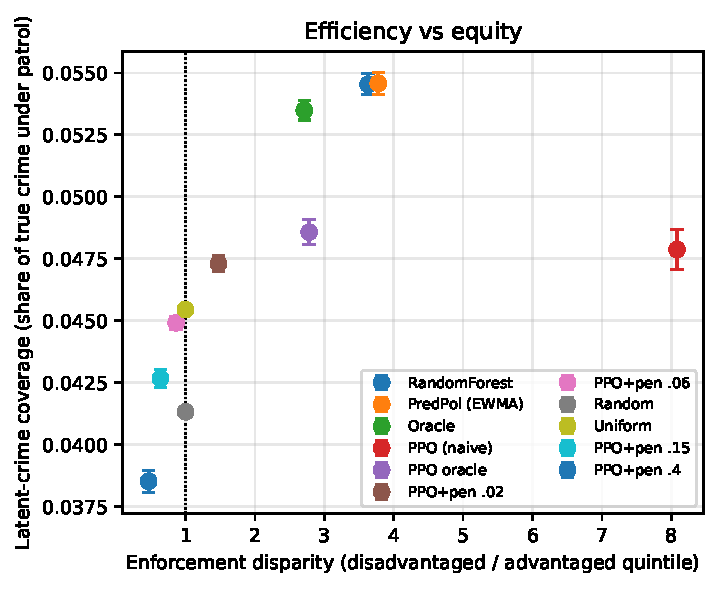
\includegraphics[width=\linewidth]{figures/fig_efficiency_equity.pdf}
\caption{E1. Enforcement disparity against latent-crime coverage. The ideal
corner is top-left. The naive PPO rule is far to the right; the penalised rules
return to parity along the frontier.}
\label{fig:effeq}
\end{figure}

\subsection{E2: the loop runs away}
Fig.~\ref{fig:feedback} tracks four quantities over the deployment horizon. The
naive rule's cumulative enforcement Gini climbs from \num{0.44} to \num{0.50} in
the first fifteen shifts and stays there -- it concentrates far harder and faster
than the PredPol heuristic (which sits near \num{0.27}). Its patrol also sits
\emph{further} from where crime actually is: the earth-mover distance between its
deployment and the latent crime-share distribution is \num{2.3}, against
\num{1.8} for uniform and \num{0.75} for the heuristic, whose allocation does
track the (still lightly biased) record. That misdirected concentration is why
its latent coverage stays below the heuristic's throughout. The penalised rule
stays near the uniform curves.

\begin{figure}[t]\centering
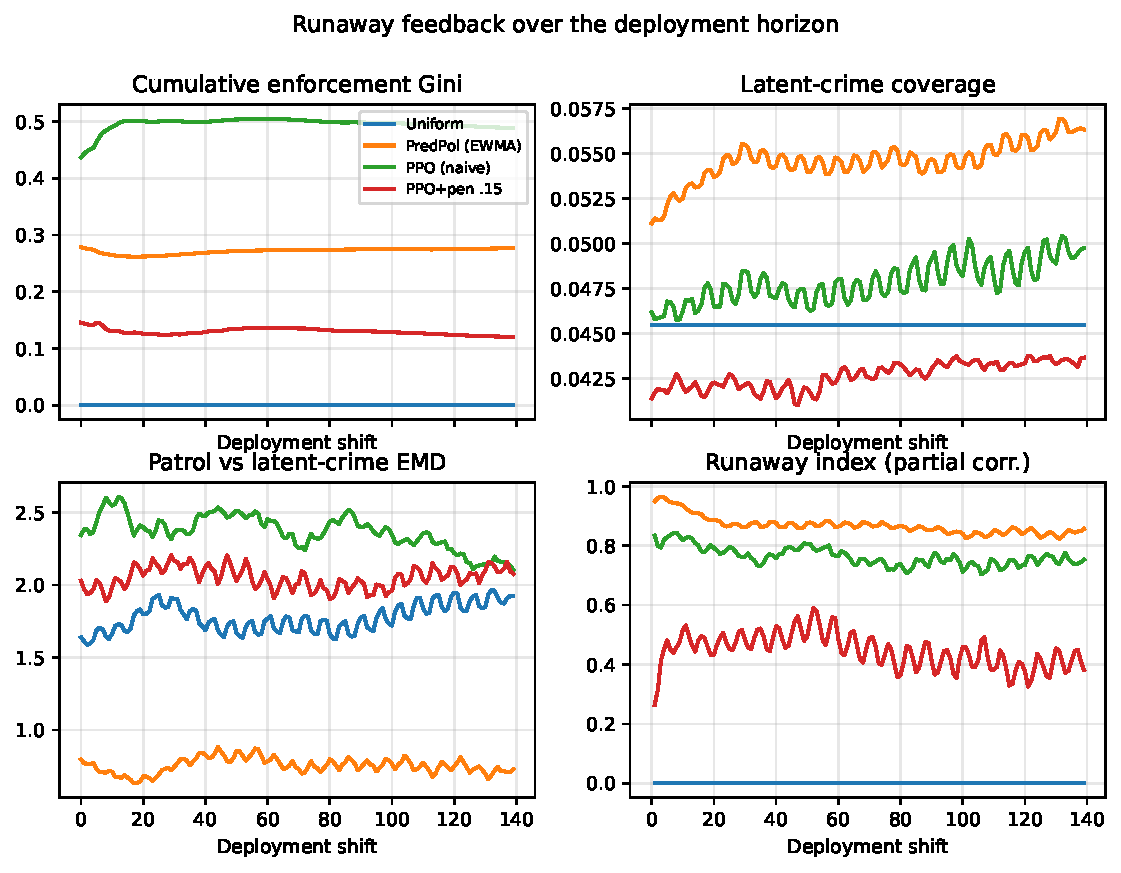
\includegraphics[width=\linewidth]{figures/fig_feedback_trajectories.pdf}
\caption{E2. Feedback quantities over the deployment horizon.}
\label{fig:feedback}
\end{figure}

\subsection{E3: the drift tracks disadvantage}
For every (policy, seed, shift, district) we form
$\text{over-policing} = a_r - L_r/\sum_{r'}L_{r'}$ and regress it on district
hardship while controlling for the district's latent crime share, with
heteroskedasticity-robust errors. A positive hardship coefficient means the
policy over-polices disadvantaged districts beyond what their true crime
justifies. The coefficient is $+0.017$ ($p < 10^{-300}$, $R^2 = 0.40$) for the
naive PPO rule -- about three times the PredPol value ($+0.005$) and twice the
latent-oracle RL ($+0.008$). The penalty drives it to zero at $w_f = 0.02$ and to
$-0.026$ at $w_f = 0.40$. Fig.~\ref{fig:incidence} plots enforcement per capita by
hardship quintile: the naive rule's exposure rises to about $3\times$ per capita
in the most-disadvantaged quintile, against $1.5$--$1.7\times$ for the heuristics,
while the penalised rule is flat.

\begin{figure}[t]\centering
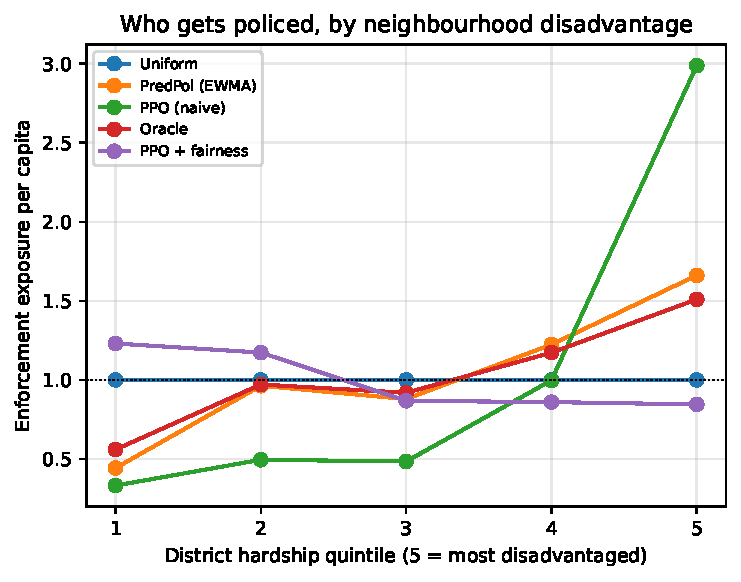
\includegraphics[width=\linewidth]{figures/fig_incidence.pdf}
\caption{E3. Enforcement exposure per capita by district hardship quintile
(5 = most disadvantaged).}
\label{fig:incidence}
\end{figure}

\subsection{E4: the penalty and the frontier}
Fig.~\ref{fig:pareto} places each policy in (disparity, latent-coverage) space
and marks the Pareto-efficient set. The naive PPO rule and the latent-oracle RL
are the only policies that are \emph{Pareto-dominated}: every heuristic and every
penalised variant reaches both higher latent coverage and lower disparity. As
$w_f$ increases the penalised rule moves monotonically along the frontier --
disparity \num{1.5}, \num{0.9}, \num{0.6}, \num{0.5}; latent coverage \num{0.047},
\num{0.045}, \num{0.043}, \num{0.039} -- with the hardship coefficient passing
through zero at the first step. The knee ($w_f = 0.02$) removes the disparity
(from \num{8.1} to \num{1.5}) and the socio-economic gradient at a latent-coverage
cost of about one percentage point relative to uniform.

\begin{figure}[t]\centering
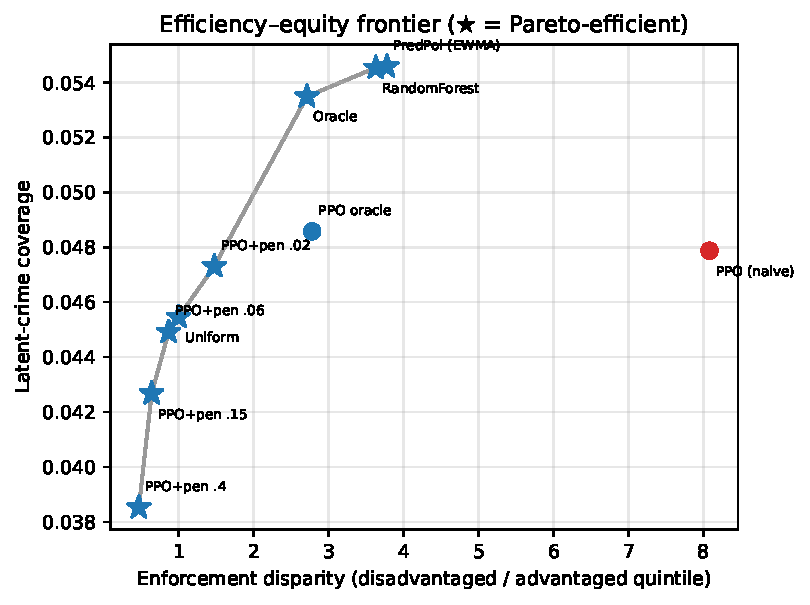
\includegraphics[width=\linewidth]{figures/fig_pareto.pdf}
\caption{E4. Efficiency--equity frontier over the fairness-penalty sweep.
Stars are Pareto-efficient.}
\label{fig:pareto}
\end{figure}

\subsection{E5: robustness}
Table~\ref{tab:e5} repeats the core comparison under six settings (single training
seed, ten held-out eval seeds). In every one the naive rule holds a large
enforcement disparity and a positive hardship coefficient while the penalised rule
holds parity and a coefficient near zero. Two interventions that remove an input
to the loop roughly halve the naive rule's disparity and hardship gradient:
turning off detection inflation (perfect observation, $q_0 = 1$ and detection gain
zero) drops the disparity from \num{9.0} to \num{2.9} and the hardship coefficient
from \num{0.036} to \num{0.018}; and removing the socio-economic covariates from
the observation drops the disparity to \num{4.3} and the coefficient to
\num{0.023}. The residual disparity under perfect observation is legitimate
targeting -- high-hardship districts do have more crime -- so the detection loop
accounts for roughly the upper half of the effect. Weak deterrence makes it worse
(disparity \num{10.7}); strong deterrence, which lets concentrated patrol actually
suppress crime and so cools the record, makes it milder (disparity \num{4.8}).

\begin{table}[t]
\caption{E5. Enforcement disparity and the E3 hardship coefficient under six
settings (naive PPO / penalised PPO). Single training seed.}
\label{tab:e5}
\centering
\begin{tabular}{lcccc}
\toprule
& \multicolumn{2}{c}{Disparity} & \multicolumn{2}{c}{Hardship coef.} \\
Setting & naive & penal. & naive & penal. \\
\midrule
Base                         & 9.0  & 0.9 & $+0.036$ & $-0.004$ \\
Perfect observation          & 2.9  & 1.0 & $+0.018$ & $-0.002$ \\
No socio-economic covariates & 4.3  & 0.9 & $+0.023$ & $-0.004$ \\
High detection gain          & 7.0  & 0.9 & $+0.028$ & $-0.006$ \\
Weak deterrence              & 10.7 & 0.5 & $+0.034$ & $-0.024$ \\
Strong deterrence            & 4.8  & 0.9 & $+0.025$ & $-0.005$ \\
\bottomrule
\end{tabular}
\end{table}

\section{Discussion}

The naive rule is not failing to solve its problem. Given the objective of
covering recorded crime, a sharp concentration on recorded hotspots is correct.
The difficulty is that this objective and the social objective -- cover real
crime, with enforcement spread in proportion to need -- come apart once the rule
can influence the record, and an RL optimiser presses on the gap harder than a
moving-average heuristic does. The extra pressure lands on the districts that are
already worst off, and the rule learns an explicit tilt in that direction.

Our claims concern a simulated world. The value of the simulator is a clean
counterfactual, not a match to Chicago's crime totals; the same limitation
applies to~\cite{ensign2018, fairsense2025, algorithms2026}. The parameters that
set the strength of the loop are swept in E5; the perfect-observation control
attributes roughly the upper half of the effect to the detection channel, the
remainder being legitimate targeting of districts that do have more crime. For a
deployed system the reading is
twofold: an allocator that trains on discovered incidents should be scored
against an instrumented estimate of latent crime rather than discovered crime,
and it should carry an explicit constraint on enforcement exposure per capita;
the penalty here is one inexpensive way to add that constraint.

\textbf{Limitations.} A coarse grid and zone-based movement; residential
population assumed uniform across districts; non-adaptive offenders (a
two-sided-learning extension has prior art in~\cite{wise2024}); parametric
deterrence and detection not calibrated to an external estimate of the reporting
rate; and a task with limited room for cleverness, so an RL oracle only matches
rather than beats the reactive heuristic on coverage.

\section{Conclusion}
Inside an unseeded, theory-grounded crime simulator in which the true crime
process is known, a reinforcement-learned patrol-allocation rule trained on the
operational objective of predictive policing learns a strong recorded-crime
concentration and an explicit tilt toward the most disadvantaged districts. It
posts the best recorded coverage of any method while covering the least actual
crime among targeted policies, and it over-polices district hardship at several
times the rate of a PredPol-style heuristic. A swept fairness penalty removes the
distortion along a monotone frontier. Because the simulator injects no historical
crime, the distortion belongs to the learned rule in a feedback loop, not to its
training data.

\section*{Acknowledgment}
We thank PES University and the Department of Computer Science and Engineering
(AI \& ML). This work was carried out as Capstone Project Phase 2 (UE23AM320B).

\bibliographystyle{IEEEtran}
\bibliography{refs}

\end{document}
